% TrialSpec-LM: IEEE conference-format report for GenAI Assignment #2.
% Build: cd report && latexmk -pdf main.tex   (or upload report/ to Overleaf)
% Figures are regenerated from committed results with: python -m src.report.figures
\documentclass[conference]{IEEEtran}
\IEEEoverridecommandlockouts
\usepackage[T1]{fontenc}
\usepackage{amsmath,amssymb}
\usepackage{graphicx}
\usepackage{booktabs}
\usepackage{multirow}
\usepackage{xcolor}
\usepackage{tikz}
\usetikzlibrary{arrows.meta,positioning,fit}
\usepackage[hidelinks]{hyperref}
\usepackage{cite}
\graphicspath{{figures/}}

% ---------------- author details: edit these ----------------
\newcommand{\authorname}{Muhammad Umair}           % TODO: check spelling
\newcommand{\rollno}{Roll No.\ XXXX}               % TODO: fill in
\newcommand{\affil}{FAST-NUCES}                    % TODO: check
\newcommand{\repourl}{https://github.com/Umairishuman/TrialSpec-LM}
% -------------------------------------------------------------

\begin{document}

\title{TrialSpec-LM: A Fine-Tuned Small Transformer for Evidence-Grounded Clinical-Trial Criterion Matching, with Hand-Written KV Caching, Tiled Attention and Speculative Decoding}

\author{\IEEEauthorblockN{\authorname\ (\rollno)}
\IEEEauthorblockA{Generative AI, Assignment 2 \\ \affil \\ Code: \url{\repourl}}}

\maketitle

\begin{abstract}
We fine-tune Qwen2.5-1.5B-Instruct with LoRA to decide, for one patient note and one clinical-trial criterion, an eligibility label from the TrialGPT annotation scheme and the IDs of the note sentences that support it. On the prescribed patient-grouped split (37/8/8 patients), the final model reaches 0.738 accuracy and 0.660 macro-F1 on the held-out test set, against 0.136 and 0.131 for the same model before fine-tuning, with an evidence micro-F1 of 0.544, no hallucinated sentence IDs and no unparseable outputs. Model selection used validation only; the test set was evaluated once. Around the model we implement, from scratch and with tests, a KV-cached greedy decoder (up to 9.3$\times$ faster decoding than the uncached reference on a T4), a tiled online-softmax attention (numerically equivalent to the reference, with linear instead of quadratic memory) and greedy speculative decoding with a 0.5B draft (token-identical to greedy, but 0.61--0.80$\times$ the speed, which we explain quantitatively). A local browser application exposes screening, evidence, an explicit rule-based patient-level aggregation and live decoding benchmarks. The main remaining weakness is the ``not enough information'' class for exclusion criteria, which reflects an inconsistency in how experts label silent notes.
\end{abstract}

\begin{IEEEkeywords}
clinical trial matching, LoRA, small language models, evidence extraction, KV cache, online softmax, speculative decoding
\end{IEEEkeywords}

% =====================================================================
\section{Introduction}
Recruiting patients is a major bottleneck of clinical trials: each trial lists many inclusion and exclusion criteria, and checking them against free-text records is slow. TrialGPT~\cite{trialgpt} showed that large language models (LLMs) can judge criteria one by one and point to supporting sentences, but it relied on GPT-4. This project asks whether a \emph{small, open-weight, locally runnable} Transformer can do the same criterion-level task with traceable evidence, and how its inference can be made efficient.

\textbf{Problem statement.} Given (i) a patient note split into numbered sentences, (ii) a criterion type (inclusion or exclusion) and (iii) the criterion text, predict one of four labels per type (inclusion: included / not included / not enough information / not applicable; exclusion: excluded / not excluded / not enough information / not applicable) and the set of sentence IDs that support the decision. The labels are \emph{not} collapsed into yes/no, and absent evidence is never treated as proof.

\textbf{Contributions.} (1) A LoRA fine-tune of Qwen2.5-1.5B with a 2$\times$2 ablation of prompt wording and rare-class oversampling, selected by validation macro-F1 (Sec.~\ref{sec:finetune}); (2) a deterministic, evidence-grounded explanation and a failure analysis of 12 test errors (Sec.~\ref{sec:results}); (3) hand-written KV-cached decoding, tiled online-softmax attention and speculative decoding, each verified against a reference (Sec.~\ref{sec:inference}); (4) a browser application with input validation, a documented aggregation rule and live benchmarks (Sec.~\ref{sec:app}). Every decision, failure and run is logged in the repository (\texttt{docs/decisions.md}, \texttt{docs/runs.md}).

% =====================================================================
\section{Related Work}
\textbf{Patient--trial matching.} The TREC/SIGIR clinical-trial collections~\cite{koopman} provide patient topics and trials; TrialGPT~\cite{trialgpt} added criterion-level expert labels and evidence sentences, the dataset used here. TrialGPT prompts GPT-4 zero-shot and reports high criterion accuracy, but depends on a proprietary API. We instead fine-tune a 1.5B open model, trading some reasoning ability for local execution and full control over decoding. GPT-4's own predictions and explanations, which ship with the dataset, are never used as inputs or targets.

\textbf{Transformers and efficient adaptation.} We use a decoder-only Transformer~\cite{vaswani} with rotary position embeddings~\cite{rope} and grouped-query attention (GQA)~\cite{gqa}, as in Qwen2.5~\cite{qwen25}. Full fine-tuning of 1.5B parameters does not fit a free 16\,GB GPU with optimiser state; LoRA~\cite{lora} trains low-rank updates of the projection matrices instead (here 18M trainable parameters, 1.2\%). QLoRA~\cite{qlora} would cut memory further with 4-bit weights, but changes the base model used for the before/after comparison, so it was not needed at 1.5B.

\textbf{Efficient inference.} Caching keys and values turns autoregressive decoding from quadratic to linear work in the sequence length; its memory cost is what dominates large-scale serving~\cite{pope}. FlashAttention~\cite{flash} computes exact attention in tiles with an online softmax~\cite{online}, avoiding the $L\times L$ score matrix. Speculative decoding~\cite{leviathan,chen} uses a cheap draft model whose proposals are verified by the target in one pass; in its greedy form the output is identical to target greedy decoding, and the speed-up depends on the acceptance rate and the draft/target cost ratio. We implement simplified versions of all three to test these claims on our model.

% =====================================================================
\section{Materials and Methods}
\subsection{Dataset and split}
The \texttt{ncbi/TrialGPT-Criterion-Annotations} dataset has 1,015 criterion annotations for 53 patients. Five columns (\texttt{gpt4\_explanation}, \texttt{gpt4\_sentences}, \texttt{gpt4\_eligibility}, \texttt{explanation\_correctness}, and the original \texttt{training} flag) are dropped at load time, and a test asserts that no \texttt{gpt4} field reaches the prompt. Patients are split exactly as prescribed: sorted IDs, NumPy \texttt{default\_rng(42)} shuffle, first 37 / next 8 / last 8. The manifest (\texttt{data/splits/split\_manifest.json}) and 9 tests check disjointness, determinism and counts. Table~\ref{tab:data} shows the resulting imbalance: ``not excluded'' alone is 48\% of all labels, ``excluded'' has 10 examples in total and none in test, and 60\% of annotations have no gold evidence. We therefore report macro-F1 as the headline metric and show per-class results with supports.

\begin{table}[t]
\centering
\caption{Split sizes and label counts (patients are disjoint).}
\label{tab:data}
\footnotesize
\begin{tabular}{lrrr}
\toprule
 & Train & Val & Test \\
\midrule
Patients / annotations & 37 / 603 & 8 / 206 & 8 / 206 \\
Empty gold evidence & 349 & 116 & 145 \\
\midrule
Incl.: included / not incl. & 88 / 13 & 35 / 3 & 27 / 7 \\
Incl.: NEI / N/A & 109 / 5 & 27 / 1 & 38 / 3 \\
Excl.: excluded / not excl. & 8 / 292 & 2 / 101 & 0 / 91 \\
Excl.: NEI / N/A & 65 / 23 & 26 / 11 & 28 / 12 \\
\bottomrule
\end{tabular}
\end{table}

\subsection{Model selection}
Table~\ref{tab:models} compares the candidates. Qwen2.5-1.5B-Instruct (Apache-2.0) fits a Kaggle T4 in fp16 with LoRA and gradient checkpointing, and Qwen2.5-0.5B-Instruct shares its tokenizer exactly (same 151,936-entry vocabulary and special tokens, checked in code), which speculative decoding requires. Qwen2.5-3B was rejected because its licence is not Apache-2.0 (Qwen Research licence) and it leaves little T4 headroom; Llama-3.2 was rejected because it is gated, and its 1B/3B pair would also work as target/draft. GQA with 2 KV heads makes the 1.5B model's KV cache only $2\cdot28\cdot2\cdot128\cdot2 = 28$\,KiB per token in fp16, 6$\times$ less than full multi-head attention.

\begin{table}[t]
\centering
\caption{Decoder candidates (from model cards and configs).}
\label{tab:models}
\footnotesize
\setlength{\tabcolsep}{3pt}
\resizebox{\columnwidth}{!}{%
\begin{tabular}{lrrrll}
\toprule
Model & Params & Layers & Q/KV heads & Licence & Role \\
\midrule
Qwen2.5-0.5B-Instr. & 0.49B & 24 & 14/2 & Apache-2.0 & draft \\
\textbf{Qwen2.5-1.5B-Instr.} & 1.54B & 28 & 12/2 & Apache-2.0 & \textbf{target} \\
Qwen2.5-3B-Instr. & 3.09B & 36 & 16/2 & Qwen Research & rejected \\
Llama-3.2-1B/3B-Instr. & 1.2/3.2B & 16/28 & 32/8, 24/8 & gated & rejected \\
\bottomrule
\end{tabular}}
\\[2pt]
\raggedright\scriptsize All Qwen2.5 models: 32k context, 151,936-token vocabulary. fp16 weights of the 1.5B model: 2.9\,GiB.
\end{table}

\subsection{Input/output format and training objective}
\label{sec:finetune}
The prompt (system instruction + note with its original sentence IDs + criterion type + criterion text + allowed labels) is rendered with the Qwen chat template. The target is the JSON \texttt{\{"evidence\_ids": [...], "label": "..."\}}, with evidence first so the label is generated conditioned on the cited sentences. The dataset has no expert explanations and GPT-4's are forbidden, so the model is \emph{not} trained to write explanations; instead an explanation is composed deterministically from the label and the exact cited sentences (e.g. ``The note indicates the patient meets this inclusion criterion, based on sentence [0] `\ldots'\,''), and when nothing is cited it says the label ``rests on the absence of reported information''. The loss is computed only on answer tokens (prompt labels set to $-100$). Prompts are 227--597 tokens with \texttt{max\_len}\,=\,1024, so \textbf{no example is truncated} and no gold evidence sentence is lost; the code raises an error rather than truncating silently.

\textbf{Training configuration.} LoRA $r{=}16$, $\alpha{=}32$, dropout 0.05 on all attention and MLP projections; learning rate $2{\times}10^{-4}$, cosine schedule, 5\% warm-up, 3 epochs, effective batch 16 ($4\times4$ accumulation), fp16 mixed precision on a Tesla T4 (no bf16 on Turing), seed 42. Each epoch is checkpointed, and the checkpoint with the highest \emph{validation macro-F1 from generated predictions} is kept: in two runs validation loss chose a worse checkpoint, because the label is only 2--5 of the 12--38 answer tokens. Training curves (W\&B, exported by script) are in Fig.~\ref{fig:curves}.

\textbf{Ablation.} Four runs cross two choices: prompt v1 (label names only) vs v2 (one-line label definitions), and no oversampling vs oversampling rare (type, label) groups to 60 rows, capped at 4$\times$.

\begin{figure}[t]
\centering
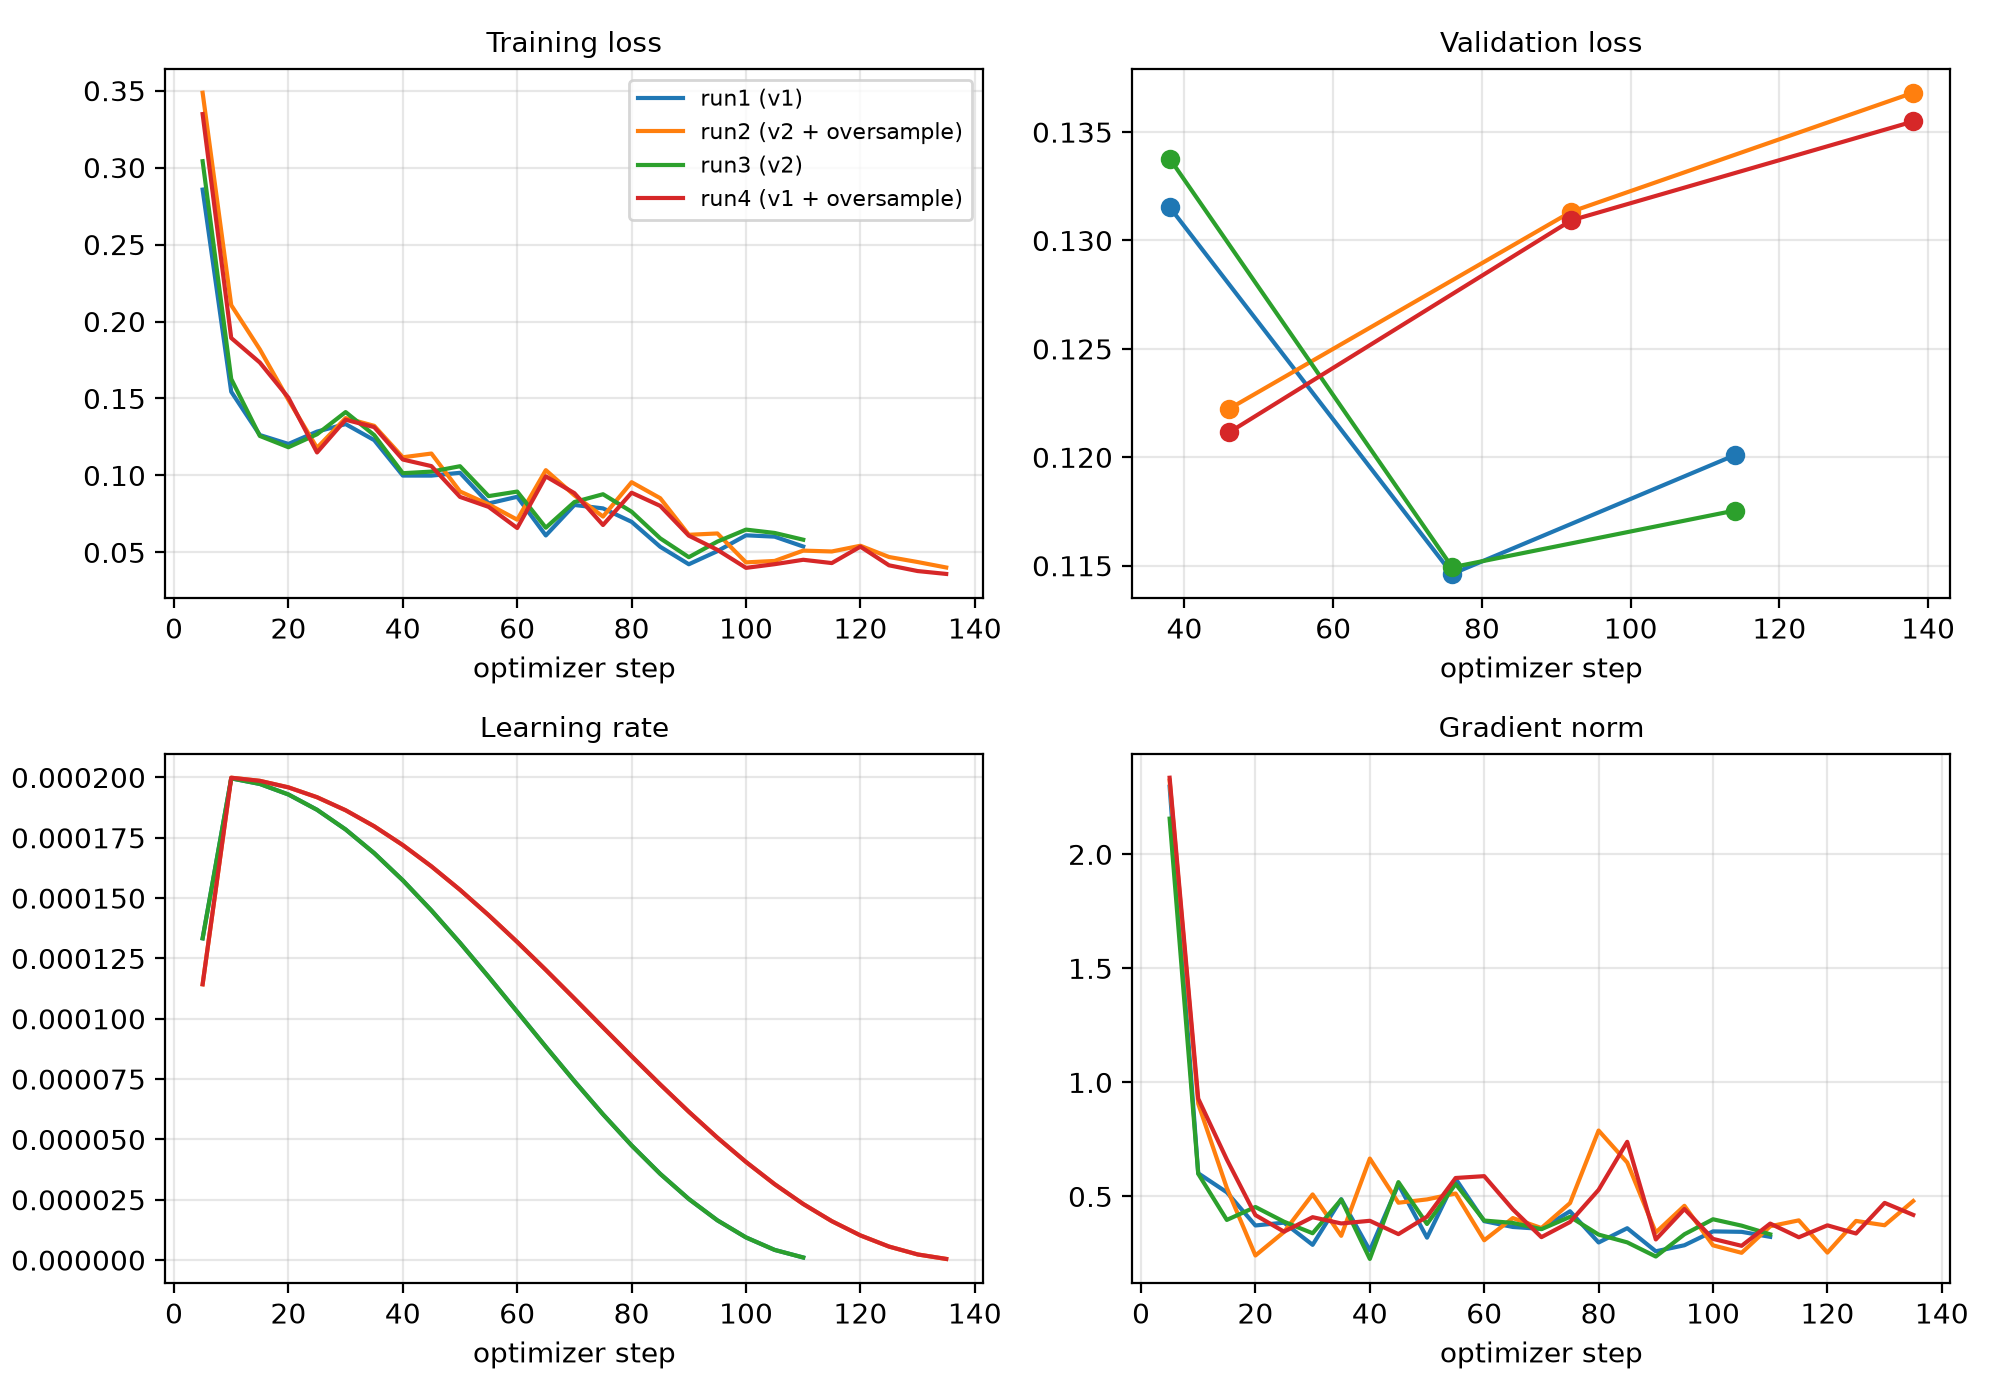
\includegraphics[width=\columnwidth]{fig_training_curves.png}
\caption{Training curves of runs 1--4. Validation loss is lowest after epoch 1 for both oversampling runs (2, 4) and then rises as repeated rare examples are memorised, yet run 4's epoch 3 has the best validation macro-F1.}
\label{fig:curves}
\end{figure}

\subsection{Pipeline overview}
Fig.~\ref{fig:pipeline} shows the full workflow: training on Kaggle, selection on validation, a single test evaluation, and the local application.

\begin{figure}[t]
\centering
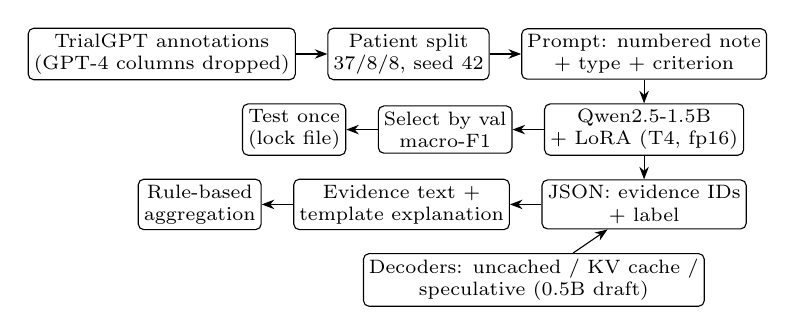
\begin{tikzpicture}[node distance=3mm and 4mm, every node/.style={font=\scriptsize}, box/.style={draw, rounded corners=2pt, align=center, minimum height=6mm, inner sep=2pt}, ar/.style={-{Stealth[length=1.6mm]}}]
\node[box] (data) {TrialGPT annotations\\(GPT-4 columns dropped)};
\node[box, right=of data] (split) {Patient split\\37/8/8, seed 42};
\node[box, right=of split] (prompt) {Prompt: numbered note\\+ type + criterion};
\node[box, below=of prompt] (lora) {Qwen2.5-1.5B\\+ LoRA (T4, fp16)};
\node[box, left=of lora] (sel) {Select by val\\macro-F1};
\node[box, left=of sel] (test) {Test once\\(lock file)};
\node[box, below=of lora] (json) {JSON: evidence IDs\\+ label};
\node[box, left=of json] (expl) {Evidence text +\\template explanation};
\node[box, left=of expl] (agg) {Rule-based\\aggregation};
\node[box, below=of json, xshift=-14mm] (dec) {Decoders: uncached / KV cache /\\speculative (0.5B draft)};
\draw[ar] (data) -- (split); \draw[ar] (split) -- (prompt); \draw[ar] (prompt) -- (lora);
\draw[ar] (lora) -- (sel); \draw[ar] (sel) -- (test); \draw[ar] (lora) -- (json);
\draw[ar] (json) -- (expl); \draw[ar] (expl) -- (agg); \draw[ar] (dec) -- (json);
\end{tikzpicture}
\caption{System overview. The top row is offline training/evaluation; the bottom rows are the inference path used by the evaluation and the application.}
\label{fig:pipeline}
\end{figure}

\subsection{Inference mechanisms}
\label{sec:inference}
All three are implemented on top of the model's weights in \texttt{src/decoding} and \texttt{src/attention}, without \texttt{generate()}.

\textbf{KV-cached decoding (Task 3).} A hand-written Qwen2 forward pass (RMSNorm, RoPE, GQA, SwiGLU MLP) keeps a preallocated cache of shape $[B, n_{kv}, \text{capacity}, d]$ per layer for keys and values. Prefill runs the whole prompt once and writes positions $[0,T)$. Each decode step feeds only the newest token, at absolute position $p = $ cache length: RoPE is applied to the new key at $p$ \emph{before} it is written, so cached keys are never re-rotated. A single query may attend to every cached key, so no mask is needed during decoding; prefill uses a causal mask with offset $L_k - L_q$, which covers both phases with one attention function. The cache grows linearly: $2 \cdot n_\text{layers} \cdot n_{kv} \cdot d \cdot \text{bytes}$ per token. We also implement an explicit loop over the HF forward with a \texttt{DynamicCache}. The reference recomputes the full sequence every step.

\textbf{Tiled attention with online softmax (Task 4).} For each query block, key/value blocks are visited in order while keeping a running maximum $m$, normaliser $\ell$ and unnormalised output $O$:
\begin{equation}
\begin{aligned}
m' &= \max\big(m, \max\nolimits_j s_j\big),\\
\ell' &= e^{m-m'}\,\ell + \textstyle\sum_j e^{s_j-m'},\\
O' &= e^{m-m'}\,O + \textstyle\sum_j e^{s_j-m'}\, v_j,
\end{aligned}
\end{equation}
and the result is $O/\ell$. Tiles entirely above the causal diagonal are skipped, and only diagonal tiles are masked. Accumulation is in fp32 for fp16 inputs.

\textbf{Greedy speculative decoding (Task 5).} Both models keep their own manual KV cache. Each round, the draft proposes $k$ tokens greedily; the target scores $[\text{last}, d_1..d_k]$ in \emph{one} forward pass; the longest prefix with $d_{i+1} = \arg\max p_i$ is accepted, followed by the target's own token (a correction, or a bonus token when all $k$ match). Both caches are then cropped back to the committed length; if all $k$ were accepted, the draft is fed $d_k$, which it has not yet processed. The output is identical to target greedy decoding by construction.

\textbf{Decoding settings.} Qwen2.5 ships a generation config with sampling parameters and \texttt{repetition\_penalty}\,=\,1.1, which \texttt{generate(do\_sample=False)} still applies. All final numbers therefore use an explicit configuration: greedy, one beam, repetition penalty 1.0, at most 64 new tokens, stop at \texttt{<|im\_end|>}. Re-scoring every model this way changed 1 of 1,236 validation outputs and no labels.

\subsection{Metrics}
Labels: accuracy, macro-F1 over the classes present in the gold labels of a subset, per-class P/R/F1 and confusion matrices, overall and separately for inclusion and exclusion. Evidence: set-based P/R/F1 over sentence IDs; when both sets are empty a record scores 1 (macro only), when exactly one is empty it scores 0; micro-averaging pools TP/FP/FN, so empty--empty records do not count. Because 145 of 206 test gold sets are empty, macro evidence F1 is inflated and micro-F1 is our main evidence metric. Cited IDs that do not exist in the note are removed and counted.

% =====================================================================
\section{Experimental Setup}
Training, evaluation and GPU benchmarks ran on Kaggle (Tesla T4, 16\,GB, PyTorch 2.11 + CUDA 13.0, Transformers 5.22.1, PEFT 0.21.2) from the GitHub repository; notebooks only call scripts, and every script has a \texttt{-{}-smoke} mode that was run before each long job. The application and CPU checks ran on a laptop (Intel i5-1145G7, 4 cores, 16\,GB RAM, no GPU, PyTorch 2.15 CPU). Benchmarks use warm-up runs, \texttt{torch.cuda.synchronize()} around timed regions, and the median or mean of repeated runs (3 for decoding, 10 for attention). The test split was used exactly once, after selection on validation, and is guarded by a committed lock file. The project has 173 automated tests (split integrity, prompt/metric functions, attention equality, KV-cache and speculative token equality on tiny random models, application logic).

% =====================================================================
\section{Results and Discussion}
\label{sec:results}
\subsection{Model selection on validation}
Table~\ref{tab:val} reports all six models on validation. Fine-tuning lifts accuracy from 7--18\% to 70--74\%. The untuned model cites no evidence at all and mostly predicts ``not applicable''; label definitions (v2) help it slightly. After fine-tuning, however, v2 hurts: its definition of ``not excluded'' (``\ldots or gives no sign of it'') erases the boundary with ``not enough information'', and runs 2--3 predict ``not excluded'' for almost every exclusion criterion. Oversampling helps only with v1 (run 4): exclusion macro-F1 rises from 0.401 to 0.676. Part of the overall gain (0.432$\to$0.604) comes from the two validation ``excluded'' cases becoming correct, which alone is worth $\approx$0.12 of macro-F1; the more robust gain is exclusion NEI F1 (0.294$\to$0.410, $n{=}26$). Run 4 was selected by the rule fixed in advance.

\begin{table}[t]
\centering
\caption{Validation results ($n{=}206$, greedy, repetition penalty 1.0).}
\label{tab:val}
\footnotesize
\setlength{\tabcolsep}{3.2pt}
\begin{tabular}{llrrrrr}
\toprule
Model & Prompt / data & Acc & mF1 & Incl. & Excl. & Ev.\,F1$_\mu$ \\
\midrule
Zero-shot & v1 & .068 & .054 & .064 & .074 & .000 \\
Zero-shot & v2 & .175 & .070 & .111 & .097 & .000 \\
Run 1 & v1 & .743 & .432 & .360 & .401 & .554 \\
Run 2 & v2 + oversample & .704 & .335 & .343 & .210 & .468 \\
Run 3 & v2 & .728 & .379 & .374 & .252 & .556 \\
\textbf{Run 4} & \textbf{v1 + oversample} & \textbf{.743} & \textbf{.604} & .368 & \textbf{.676} & .520 \\
\bottomrule
\end{tabular}
\end{table}

\subsection{Held-out test results}
Table~\ref{tab:test} gives the single test evaluation, before and after fine-tuning on identical examples and decoding. Accuracy rises from 0.136 to 0.738 and macro-F1 from 0.131 to 0.660 (7 classes; ``excluded'' has no test examples and is reported as N/A). Every output was valid JSON with an allowed label, and no hallucinated sentence ID was produced. Test and validation macro-F1 differ by 0.056, within the noise expected from 8 patients per split.

\begin{table}[t]
\centering
\caption{Test results ($n{=}206$, evaluated once). Per-class F1 (support) for the fine-tuned model.}
\label{tab:test}
\footnotesize
\setlength{\tabcolsep}{3.5pt}
\resizebox{\columnwidth}{!}{%
\begin{tabular}{lrrrrrr}
\toprule
Model & Acc & mF1 & Incl. & Excl. & Ev.\,P/R/F1$_\mu$ & Ev.\,F1$_M$ \\
\midrule
Zero-shot v1 & .136 & .131 & .158 & .132 & .00/.00/.000 & .704 \\
\textbf{Run 4} & \textbf{.738} & \textbf{.660} & \textbf{.664} & \textbf{.514} & .46/.66/\textbf{.544} & .778 \\
\midrule
\multicolumn{7}{l}{Incl.: included .863 (27), not included .429 (7), NEI .864 (38), N/A .500 (3)}\\
\multicolumn{7}{l}{Excl.: excluded N/A (0), not excluded .816 (91), \textbf{NEI .154 (28)}, N/A .571 (12)}\\
\bottomrule
\end{tabular}}
\end{table}

Fig.~\ref{fig:cm} shows where the errors are. Inclusion is strong. The weak cell is exclusion NEI: 23 of 28 such criteria are predicted ``not excluded''. This is not random: in the training data 75\% of ``not excluded'' labels cite no sentence, i.e.\ experts usually treat an unreported excluding condition as absent, yet sometimes label the same situation NEI. The model learns the majority convention. This is exactly the case the assignment warns about (absent evidence is not proof), so the application flags every decision without cited evidence (Sec.~\ref{sec:app}).

\begin{figure}[t]
\centering
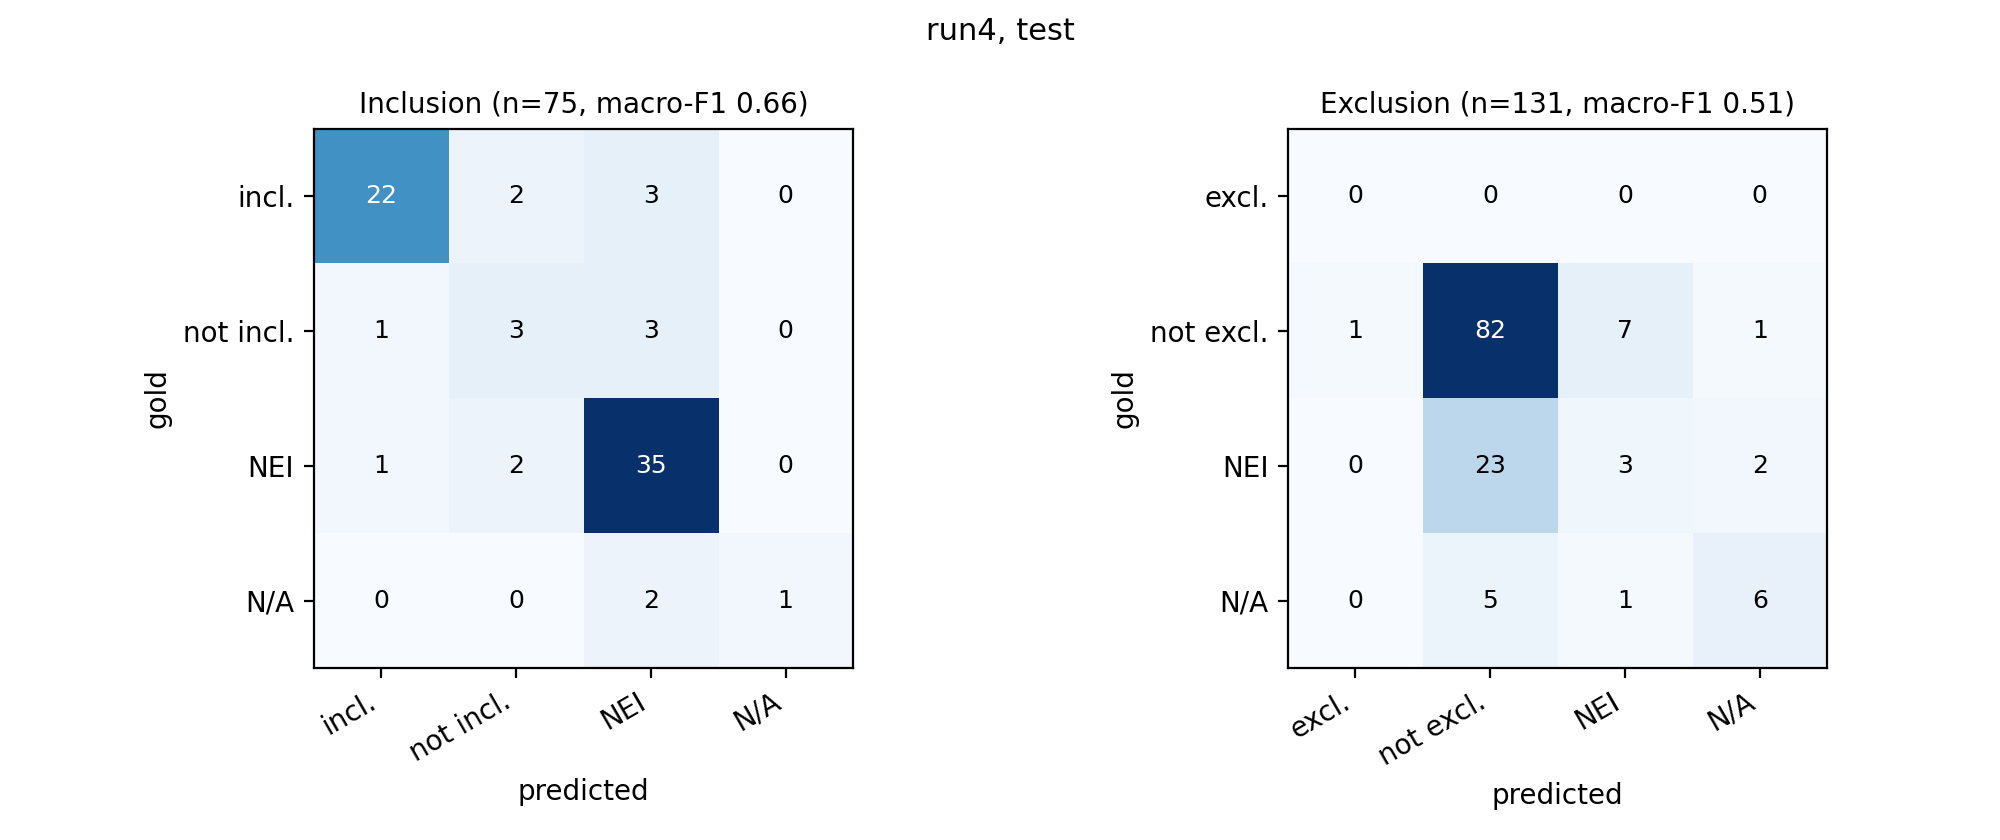
\includegraphics[width=\columnwidth]{fig_confusion_run4_test.png}
\caption{Test confusion matrices of the final model (rows: gold). Exclusion NEI is mostly predicted as ``not excluded''.}
\label{fig:cm}
\end{figure}

\subsection{Error analysis}
Of 206 test predictions, 54 labels are wrong. Automatic categories: missed information (gold NEI, definite prediction) 28; spurious NEI 16; applicability confusions 6; polarity flips 4; correct label with evidence not overlapping the gold set 30; hallucinated IDs and parse failures 0. We read 12 sampled cases in full (\texttt{results/final/error\_analysis\_test.md}) and found seven recurring causes:
(1)~\emph{silent-note convention}: e.g.\ ``previous axillary surgery'' is never mentioned; experts say NEI, the model ``not excluded''; the reverse also occurs (``maintenance haemodialysis'': experts infer ``not included'', the model abstains);
(2)~\emph{clinical inference from raw findings}: for a patient with BP 80/60, tachycardia and tachypnoea, the model cites the right sentences but does not conclude ``shock'' (gold: included) or ``possibly moribund'' (gold: NEI);
(3)~\emph{numeric thresholds}: ``excruciating pain'' is judged ``not included'' for ``pain $\ge$\,3/10'' although the right sentence is cited; the same failure appeared on an unseen note in the app (HbA1c 8.1\% vs ``7--10\%'');
(4)~\emph{compound criteria}: ``immune deficiency \emph{and} early bone-marrow failure'', with the first part confirmed and the second unknown, is answered ``not included'' instead of NEI;
(5)~\emph{surface matching}: a femoral-artery complication is matched to ``undergoing lower-limb revascularisation'';
(6)~\emph{vague criteria and oversampling}: ``other inappropriate situation'' is answered ``excluded''; oversampling the 8 training ``excluded'' examples makes such answers likelier, the price of run 4's gains;
(7)~\emph{metric limits}: several ``unsupported evidence'' cases cite a sensible sentence (the procedure the patient actually had) where experts cited none, so 30 is an upper bound.
Causes (1), (4) and (6) are partly properties of the labels rather than of the model.

\subsection{KV cache}
On the fine-tuned model in fp16 on the T4, the cached paths reproduce the uncached reference token for token in 16 of the 18 (cached mode, length) combinations (inputs 128/512/1024 $\times$ outputs 32/128/256). The two mismatches (hand-written cache, input 128) start at the same step, where the reference's top-1 and top-2 logits are \emph{exactly} equal in fp16 (margin 0.000); the cached path computes the same attention with a different reduction order, so the tie breaks the other way. The same code is token-exact in fp32/fp64. Fig.~\ref{fig:kv} shows the effect of caching: cached decoding is flat at $\approx$26 tokens/s regardless of prompt length, while uncached decoding falls from 15 to 2.8 tokens/s as every step reprocesses the sequence, a 9.3$\times$ speed-up at 1024+256 tokens. Caching also lowers peak memory, because the uncached path recomputes activations for the whole sequence; the cache itself is 35\,MiB at 1,280 tokens, matching the 28\,KiB/token formula. The hand-written decoder is within 3--4\% of HF's cached path. Prefill time is identical across modes (41/120/285\,ms for 128/512/1024 tokens), as expected.

\begin{figure}[t]
\centering
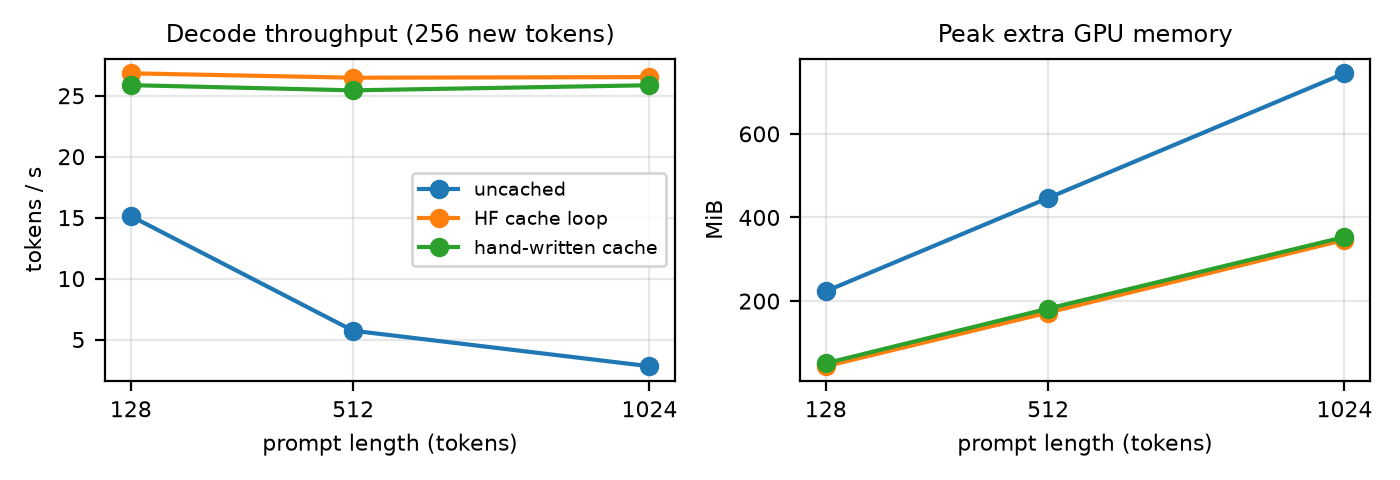
\includegraphics[width=\columnwidth]{fig_kv_cache.png}
\caption{KV-cache benchmark (T4, fp16, 256 new tokens, mean of 3 runs after warm-up).}
\label{fig:kv}
\end{figure}

\subsection{Tiled attention}
52 unit tests cover six shapes (lengths 1--130, including single-token decode against a 97-key cache and chunked prefill, head dims 8--128), block sizes 16$\times$16, 64$\times$32 and 7$\times$13, causal and non-causal masks, in fp64 (agreement to $10^{-10}$), fp32 and fp16. In the benchmark (lengths 128--4096) against an fp64 ground truth on the T4, the maximum error is $1.2\times10^{-6}$ in fp32 and $\le 1.7\times10^{-3}$ in fp16, identical to the reference and to PyTorch's fused SDPA (this is fp16 output rounding). Fig.~\ref{fig:att} shows the trade-off: the reference materialises the $B\!\cdot\!H\!\cdot\!L^2$ score matrix (2.3\,GB at $L{=}4096$), while the tiled version's extra memory grows linearly (14\,MiB), like the fused kernel. It is, however, 10$\times$ slower than the reference and 70--135$\times$ slower than fused SDPA on the GPU. Each tile issues several separate CUDA kernels from a Python loop (about 30k launches at $L{=}4096$), and every intermediate goes through GPU memory; a fused kernel does the same online softmax in one launch with tiles kept in on-chip SRAM. Skipping masked tiles halves the causal time (1233$\to$652\,ms).

\begin{figure}[t]
\centering
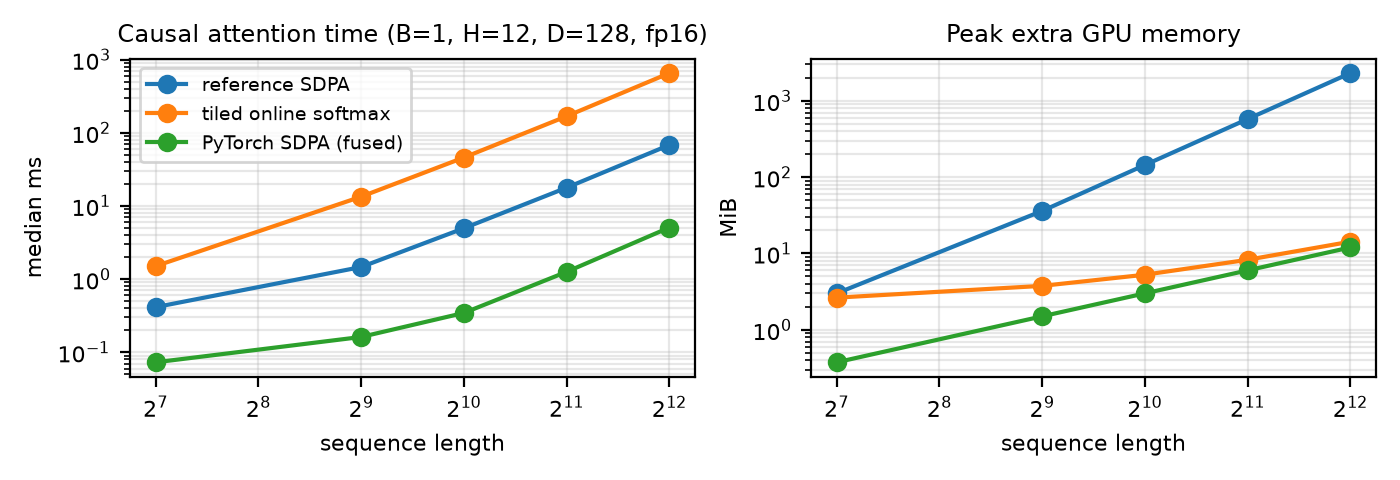
\includegraphics[width=\columnwidth]{fig_attention.png}
\caption{Attention benchmark (T4, fp16, causal, median of 10 runs; log scales).}
\label{fig:att}
\end{figure}

\subsection{Speculative decoding}
All 64 speculative runs on 16 validation-derived prompts are token-identical to target greedy decoding, and HF's own assisted generation agrees once pure greedy is enforced. Acceptance is high on task prompts even though the draft is not fine-tuned (0.72--0.83; the JSON scaffold is easy to guess) and falls with $k$ on free text (0.76$\to$0.49), Fig.~\ref{fig:spec}. Yet decoding is 0.61--0.80$\times$ the speed of plain greedy. The reason is that batch-1 decoding on the T4 is \emph{launch-bound}: a cached 1.5B step takes $\approx$37\,ms, about 4$\times$ the 9\,ms needed to read its 3\,GB of weights, so cost scales with layer count rather than parameter count, and the 24-layer draft costs $c\approx24/28\approx0.86$ of a 28-layer target step. With acceptance $\alpha$, the expected speed-up~\cite{leviathan} is $S = \frac{1-\alpha^{k+1}}{(1-\alpha)(kc+1)}$; for $\alpha{=}0.79$, $k{=}4$ this predicts 0.77$\times$, and we measured 0.74$\times$. A speed-up would need $c\lesssim0.3$, i.e.\ a much shallower draft or CUDA graphs to remove launch overhead.

\begin{figure}[t]
\centering
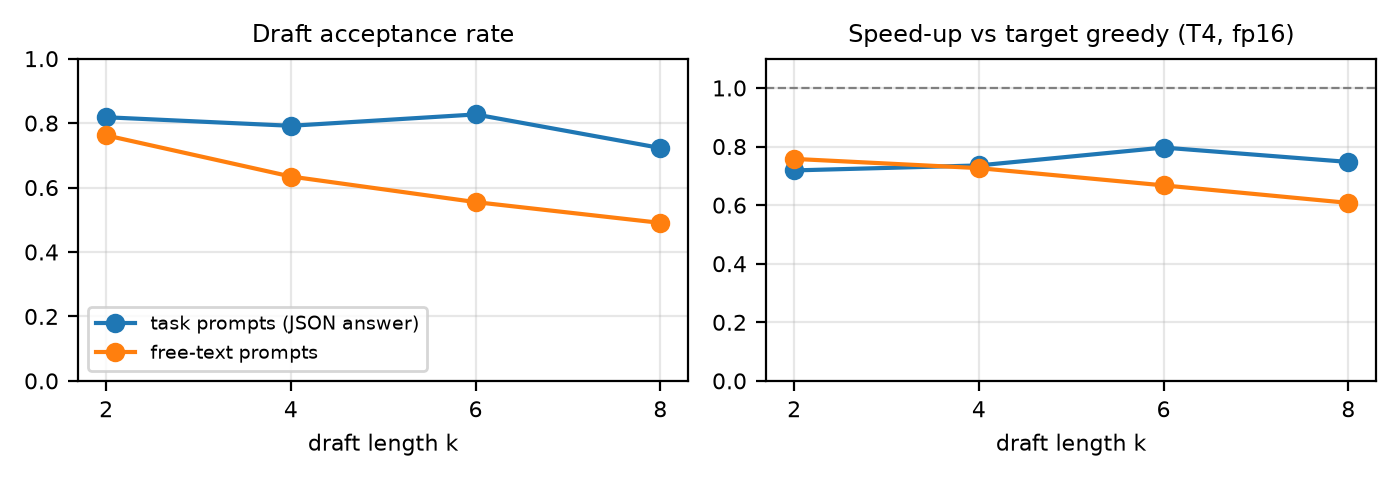
\includegraphics[width=\columnwidth]{fig_speculative.png}
\caption{Speculative decoding vs draft length $k$ (T4, fp16, 8 prompts per set, 3 repeats). Outputs are identical to greedy in all cases; the dashed line is break-even.}
\label{fig:spec}
\end{figure}

% =====================================================================
\section{Application}
\label{sec:app}
The application (\texttt{src/app}, Gradio) starts with \texttt{python -m src.app} and serves \url{http://localhost:7860}; \texttt{-{}-prefetch} downloads every model once so the demo runs offline. A user pastes a note (free text is split into numbered sentences; a note already in ``\texttt{<id>.\ sentence}'' format keeps its IDs) and enters criteria or loads an example trial from the train/validation split. Each criterion is processed with the evaluated prompt, decoding settings and parser. The results table (Fig.~\ref{fig:app}) shows the label, highlighted evidence sentences and the deterministic explanation, with flags for missing information, ``no supporting evidence cited'', invalid IDs and retries. A malformed answer is retried with a larger budget if it was cut off, then resolved by ranking the four allowed answers by model likelihood; such rows are flagged and treated as unresolved.

\textbf{Aggregation rule.} The patient-level result is explicitly a rule over model predictions, not ground truth. Inclusion ``not included'' or exclusion ``excluded'' is \emph{blocking}; ``not enough information'', fallbacks and errors are \emph{unresolved}; ``not applicable'' is ignored. Any blocking criterion gives \emph{Not eligible (preliminary)}; otherwise any unresolved criterion, or no satisfied inclusion criterion, gives \emph{Needs review}; otherwise \emph{Likely eligible (preliminary)}.

Input validation rejects empty notes or criteria, notes over 6,000 characters or 60 sentences, more than 20 criteria, and prompts over the 1,024-token training length, with readable messages. Reports export as Markdown or HTML with provenance (model, adapter and how it was selected, prompt version, decoding settings, git commit, library versions, timestamp) and the disclaimer ``Educational screening prototype --- not a clinical enrollment decision.'' A benchmark tab runs the four decoding modes live on the same prompt and reports timings, speed-ups, KV-cache size, acceptance rate and token equality.

On the laptop CPU, bf16 turned out 2.3$\times$ \emph{slower} than fp32 for prompt processing (12.6 vs 5.4\,s for 284 tokens), because this CPU has no native bf16 matrix instructions; the app therefore runs in fp32 (8\,GB RAM), at $\approx$6--13\,s per criterion. In a live test on an unseen note, three of four criteria were correct with the right evidence, and the fourth (HbA1c 8.1\% vs ``7--10\%'') was a genuine model error that the rule turned into ``Needs review''.

\begin{figure}[t]
\centering
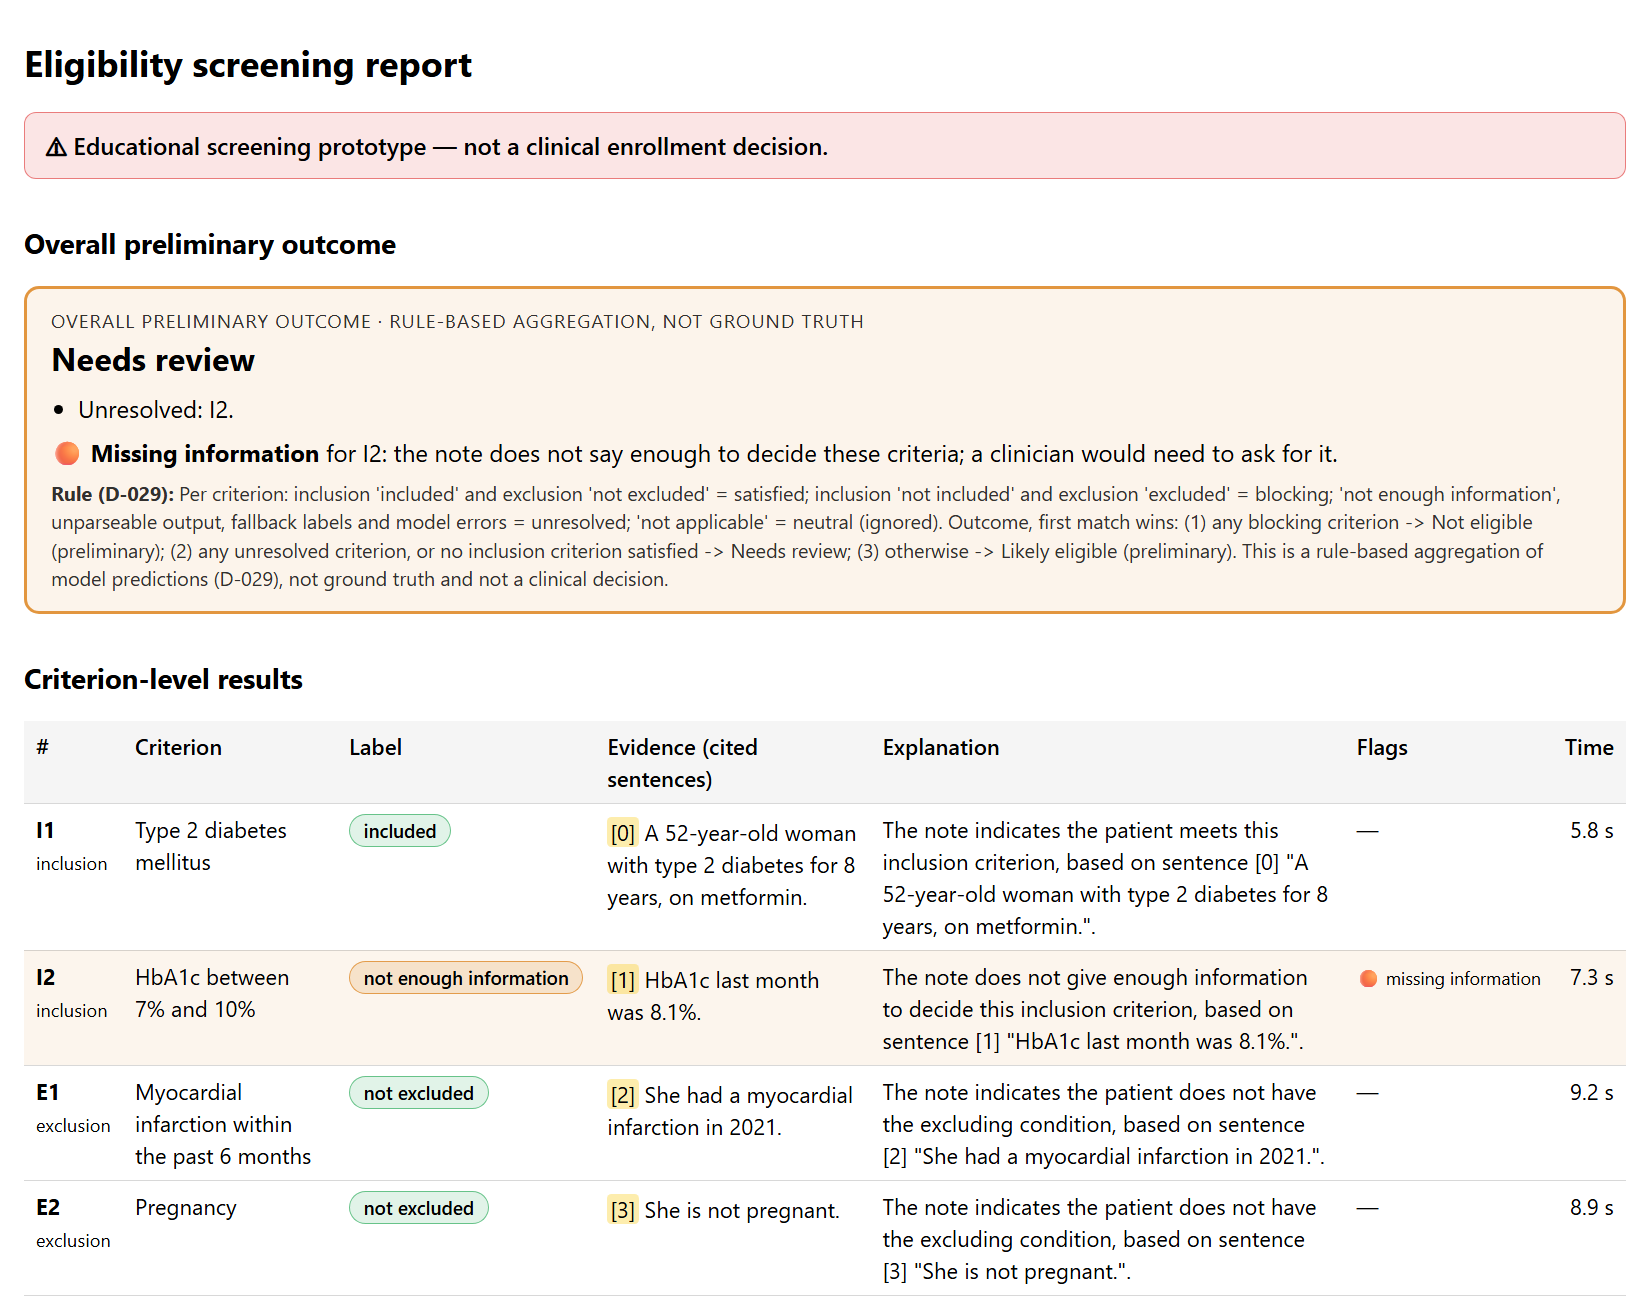
\includegraphics[width=\columnwidth]{fig_app_report.png}
\caption{Exported report for an unseen note: disclaimer, rule-based outcome with missing information, and per-criterion labels with highlighted evidence and explanations.}
\label{fig:app}
\end{figure}

\IfFileExists{figures/fig_app_ui.png}{%
\begin{figure}[t]
\centering
\includegraphics[width=\columnwidth]{fig_app_ui.png}
\caption{The application's screening tab.}
\label{fig:appui}
\end{figure}}{}

% =====================================================================
\section{Limitations}
\begin{itemize}
\item \textbf{Small, imbalanced evaluation.} Validation and test each have 8 patients; four classes have 0--7 test examples, so per-class numbers are noisy, and ``excluded'' cannot be evaluated on test at all.
\item \textbf{Label convention.} Silent notes are labelled inconsistently by the experts, which caps exclusion-NEI performance and makes ``not excluded'' predictions rest on absent information.
\item \textbf{Clinical reasoning.} A 1.5B model fails at numeric thresholds, compound criteria and inferring states from vital signs.
\item \textbf{Template explanations.} Explanations are faithful to the cited sentences but not free-text reasoning (by design, since no permitted explanation data exists).
\item \textbf{Selection confound.} Runs 1--2 were selected by loss and runs 3--4 by macro-F1; run 1's other checkpoints were not kept.
\item \textbf{Efficiency implementations are educational.} The tiled attention and speculative decoder are correct but slower than fused or launch-free implementations; the manual decoder supports batch size 1 and unscaled RoPE only.
\item \textbf{Not a clinical tool.} The system screens single criteria and has not been validated for any clinical use.
\end{itemize}

\section{Conclusion}
A LoRA-tuned 1.5B open model learns the TrialGPT criterion task from 603 examples to 0.738 accuracy and 0.660 macro-F1 on held-out patients, with grounded, checkable evidence and no format failures, and runs on a laptop CPU. The choice between prompt wordings and the use of oversampling mattered more than any other setting, and selecting checkpoints by the reported metric rather than loss was necessary. Our KV cache, tiled attention and speculative decoder reproduce the expected correctness and trade-offs, and the measurements explain when they do and do not pay off on this hardware. Future work: a fine-tuned shallow draft model, CUDA graphs for decoding, and resolving the silent-note label convention before training.

\section*{Reproducibility}
Code, configs, split manifest, results and logs: \url{\repourl}. Adapters: \url{https://huggingface.co/umairishuman/trialspec-qwen2.5-1.5b-lora-run4} (final) and runs 1--3 under the same account. W\&B project: \texttt{trialspec-lm}. Commands are listed in the README.

\appendix
\section*{AI-Use Appendix}
Claude Code (Anthropic) was used throughout as a coding assistant: drafting and refactoring code, tests and scripts; debugging failed runs (e.g.\ the Kaggle shell error, the bf16 slowdown); drafting documentation, the decision log and this report from the logged results. All runs were launched and inspected by the author; every reported number comes from committed result files produced by the project's scripts; design decisions (model, split handling, selection rule, aggregation rule) were discussed and approved by the author and are recorded with their reasoning in \texttt{docs/decisions.md}. The author reviewed the code and is able to explain and modify each component. No AI system was used to label or generate data, and GPT-4 outputs in the dataset were never used.

\begin{thebibliography}{99}
\bibitem{trialgpt} Q.~Jin, Z.~Wang, C.~S. Floudas, F.~Chen, C.~Gong, D.~Bracken-Clarke, E.~Xue, Y.~Yang, J.~Sun, and Z.~Lu, ``Matching patients to clinical trials with large language models,'' \emph{Nature Communications}, vol.~15, art.~9074, 2024.
\bibitem{koopman} B.~Koopman and G.~Zuccon, ``A test collection for matching patients to clinical trials,'' in \emph{Proc. ACM SIGIR}, 2016, pp.~669--672.
\bibitem{vaswani} A.~Vaswani, N.~Shazeer, N.~Parmar, J.~Uszkoreit, L.~Jones, A.~N. Gomez, {\L}.~Kaiser, and I.~Polosukhin, ``Attention is all you need,'' in \emph{Advances in Neural Information Processing Systems}, 2017.
\bibitem{qwen25} Qwen Team (A.~Yang \emph{et al.}), ``Qwen2.5 technical report,'' arXiv:2412.15115, 2024.
\bibitem{lora} E.~J. Hu, Y.~Shen, P.~Wallis, Z.~Allen-Zhu, Y.~Li, S.~Wang, L.~Wang, and W.~Chen, ``LoRA: Low-rank adaptation of large language models,'' in \emph{Proc. ICLR}, 2022.
\bibitem{qlora} T.~Dettmers, A.~Pagnoni, A.~Holtzman, and L.~Zettlemoyer, ``QLoRA: Efficient finetuning of quantized LLMs,'' in \emph{Advances in Neural Information Processing Systems}, 2023.
\bibitem{rope} J.~Su, Y.~Lu, S.~Pan, A.~Murtadha, B.~Wen, and Y.~Liu, ``RoFormer: Enhanced transformer with rotary position embedding,'' arXiv:2104.09864, 2021.
\bibitem{gqa} J.~Ainslie, J.~Lee-Thorp, M.~de~Jong, Y.~Zemlyanskiy, F.~Lebr{\'o}n, and S.~Sanghai, ``GQA: Training generalized multi-query transformer models from multi-head checkpoints,'' in \emph{Proc. EMNLP}, 2023.
\bibitem{pope} R.~Pope, S.~Douglas, A.~Chowdhery, J.~Devlin, J.~Bradbury, A.~Levskaya, J.~Heek, K.~Xiao, S.~Agrawal, and J.~Dean, ``Efficiently scaling transformer inference,'' in \emph{Proc. MLSys}, 2023.
\bibitem{flash} T.~Dao, D.~Y. Fu, S.~Ermon, A.~Rudra, and C.~R{\'e}, ``FlashAttention: Fast and memory-efficient exact attention with IO-awareness,'' in \emph{Advances in Neural Information Processing Systems}, 2022.
\bibitem{online} M.~Milakov and N.~Gimelshein, ``Online normalizer calculation for softmax,'' arXiv:1805.02867, 2018.
\bibitem{leviathan} Y.~Leviathan, M.~Kalman, and Y.~Matias, ``Fast inference from transformers via speculative decoding,'' in \emph{Proc. ICML}, 2023.
\bibitem{chen} C.~Chen, S.~Borgeaud, G.~Irving, J.-B. Lespiau, L.~Sifre, and J.~Jumper, ``Accelerating large language model decoding with speculative sampling,'' arXiv:2302.01318, 2023.
\end{thebibliography}

\end{document}
